\part{Appendix}

\chapter{LED Protocol}
\label{appendix/led-protocol:led-protocol}\label{appendix/led-protocol::doc}
The firmware communicates with the protocol described here. The driver sends a command with arguments ({\hyperref[appendix/led-protocol:protocol-input]{\emph{Input}}}) and the hardware send feedback on what is happening ({\hyperref[appendix/led-protocol:protocol-output]{\emph{Output}}}).


\section{Schema}
\label{appendix/led-protocol:schema}
The following schema is used for every command, in every direction:

\begin{verbatim}
cmd [arg1] [arg2] ... [argN]
\end{verbatim}


\section{Input}
\label{appendix/led-protocol:input}\label{appendix/led-protocol:protocol-input}
Commands send to the hardware


\subsection{on}
\label{appendix/led-protocol:on}\label{appendix/led-protocol:protocol-input-on}
Turns on a led:

\begin{verbatim}
on [led]
\end{verbatim}

\textbf{Arguments}
\begin{itemize}
\item {} 
\code{led} (int) - the led number

\end{itemize}


\subsection{flicker}
\label{appendix/led-protocol:flicker}\label{appendix/led-protocol:protocol-input-flicker}
Flickers a led:

\begin{verbatim}
flicker [led] [frequency] [duration] [[light]] [[dark]]
\end{verbatim}

\textbf{Arguments}
\begin{itemize}
\item {} 
\code{led} (int) - the led number

\item {} 
\code{frequency} (int) - the flicker frequency {[}hz{]}

\item {} 
\code{duration} (int) - the duration the led flickers {[}ms{]}

\item {} 
\code{light} (int) - the light part of the light/dark ratio (optional)

\item {} 
\code{dark} (int) - the dark part of the light/dark ratio (optional)

\end{itemize}


\subsection{off}
\label{appendix/led-protocol:protocol-input-off}\label{appendix/led-protocol:off}
Turns off a led:

\begin{verbatim}
off [led]
\end{verbatim}

\textbf{Arguments}
\begin{itemize}
\item {} 
\code{led} (int) - the led number

\end{itemize}


\subsection{measurement}
\label{appendix/led-protocol:protocol-input-measurement}\label{appendix/led-protocol:measurement}
Runs a measurement sequence:

\begin{verbatim}
measurement [mode] [flickerLed] [frequency] [onDuration] [offDuration]
\end{verbatim}

\textbf{Arguments}
\begin{itemize}
\item {} 
\code{mode} (int) - \emph{2} for two leds and \emph{4} for four leds

\item {} 
\code{flickerLed} (int) - Which led will flicker

\item {} 
\code{frequency} (float) - The frequency for the flickering led {[}hz{]}

\item {} 
\code{onDuration} (int) - The duration, the leds will be on {[}ms{]}

\item {} 
\code{offDuration} (int) - The duration, the leds will be off {[}ms{]}

\end{itemize}


\subsection{ping}
\label{appendix/led-protocol:ping}\label{appendix/led-protocol:protocol-input-ping}
Sends a ping:

\begin{verbatim}
ping [[seq]]
\end{verbatim}

\textbf{Arguments}
\begin{itemize}
\item {} 
\code{seq} (misc) - An optional sequence identifier (optional)

\end{itemize}


\section{Output}
\label{appendix/led-protocol:output}\label{appendix/led-protocol:protocol-output}
Feedback received from the hardware.


\subsection{on}
\label{appendix/led-protocol:protocol-output-on}\label{appendix/led-protocol:id1}
Send when a led is turned on (or flickering, when measurement command was used):

\begin{verbatim}
on [led]
\end{verbatim}

\textbf{Arguments}
\begin{itemize}
\item {} 
\code{led} (int) - the led number

\end{itemize}


\subsection{flicker}
\label{appendix/led-protocol:id2}\label{appendix/led-protocol:protocol-output-flicker}
Send when a led is flickering:

\begin{verbatim}
flicker [led]
\end{verbatim}

\textbf{Arguments}
\begin{itemize}
\item {} 
\code{led} (int) - the led number

\end{itemize}


\subsection{off}
\label{appendix/led-protocol:protocol-output-off}\label{appendix/led-protocol:id3}
Send when a led is turned off:

\begin{verbatim}
off [led]
\end{verbatim}

\textbf{Arguments}
\begin{itemize}
\item {} 
\code{led} (int) - the led number

\end{itemize}


\subsection{measurement}
\label{appendix/led-protocol:id4}\label{appendix/led-protocol:protocol-output-measurement}
Send when a measurement is started or finished:

\begin{verbatim}
measurement [state]
\end{verbatim}

\textbf{Arguments}
\begin{itemize}
\item {} 
\code{state} (string) - \code{on} when the measurement started and \code{off} when it's finished

\end{itemize}


\subsection{ons}
\label{appendix/led-protocol:ons}\label{appendix/led-protocol:protocol-output-ons}
Send when more than one led is turned on (during a measurement):

\begin{verbatim}
ons [mode]
\end{verbatim}

\textbf{Arguments}
\begin{itemize}
\item {} 
\code{mode} (int) - is either 2 or 4, depending the first value of the \code{measurement} input command

\end{itemize}


\subsection{offs}
\label{appendix/led-protocol:protocol-output-offs}\label{appendix/led-protocol:offs}
Send when more than one led is turned off (during a measurement):

\begin{verbatim}
offs [mode]
\end{verbatim}

\textbf{Arguments}
\begin{itemize}
\item {} 
\code{mode} (int) - is either 2 or 4, depending the first value of the \code{measurement} input command

\end{itemize}


\subsection{pong}
\label{appendix/led-protocol:pong}\label{appendix/led-protocol:protocol-output-pong}
Answers a ping with a pong:

\begin{verbatim}
pong [seq]
\end{verbatim}

\textbf{Arguments}
\begin{itemize}
\item {} 
\code{seq} (misc) - The returned sequence identifier (optional)

\end{itemize}


\subsection{error}
\label{appendix/led-protocol:protocol-output-error}\label{appendix/led-protocol:error}
Send when an error occured:

\begin{verbatim}
error [number]
\end{verbatim}

\textbf{Arguments}
\begin{itemize}
\item {} 
\code{number} (int) - the error number (see below)

\end{itemize}


\section{Error Codes}
\label{appendix/led-protocol:error-codes}
Error code explanation:
\begin{itemize}
\item {} 
\emph{0} - Unknown Error

\item {} 
\emph{1} - Malformed command

\item {} 
\emph{2} - Unknown command

\item {} 
\emph{3} - Too few arguments for flicker command

\end{itemize}


\section{Troubleshooting}
\label{appendix/led-protocol:troubleshooting}
1. Getting a ``Port in Use'' exception on OSX, when connecting to the Arduino Board
-\textgreater{} See here: \href{https://marcosc.com/2011/10/arduino-java-error-serial-port-already-in-use/}{https://marcosc.com/2011/10/arduino-java-error-serial-port-already-in-use/}


\chapter{ERM}
\label{appendix/erm:erm}\label{appendix/erm::doc}
The softwares database entity-relation-model (ERM) as seen in Figure~\ref{fig:appendix-erm}

\begin{figure}[H]
	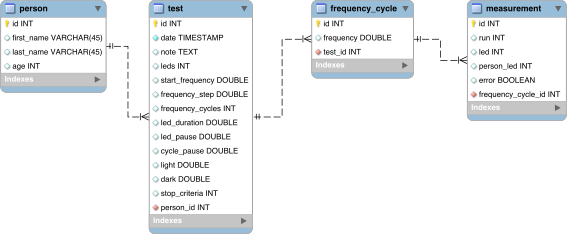
\includegraphics[width=\textwidth]{images/erm.png}
	\caption{ERM}
	\label{fig:appendix-erm}
\end{figure}

